% 第9章——中文稿件片段。
% 主文档需加载：amsmath, amssymb, booktabs, graphicx, array, xcolor；
% 中文独立编译时还需使用 XeLaTeX/LuaLaTeX 与 ctex。

\section{数值实验}
\label{sec:numerical_evaluation_zh}

\subsection{实验目标与流程}
\label{sec:evaluation_objective_zh}

本实验旨在评估：在预先设定的加速倍数与测量噪声范围内，本文提出的平滑到硬阈值谱正则化方法，能否相对于奇异值软阈值（Soft）、不连续硬阈值（Hard）以及低秩加稀疏（L+S）方法改善动态心脏 MRI 重建。四种方法使用相同的正式 OCMR 序列、采样掩膜、含噪观测、验证划分和停止准则。所有回顾性降采样和加噪均在线圈压缩、逐帧灵敏度估计和灵敏度加权线圈合成之后进行，因此实验求解的是单图像笛卡尔采样逆问题（图~\ref{fig:evaluation_pipeline_zh}）。

\begin{figure*}[t]
  \centering
  \begingroup
  \setlength{\tabcolsep}{2pt}
  \renewcommand{\arraystretch}{1.12}
  \newcommand{\pipeboxzh}[1]{\fbox{\parbox[c][1.05cm][c]{0.205\textwidth}{\centering\small #1}}}
  \resizebox{\textwidth}{!}{%
  \begin{tabular}{c@{\;${\longrightarrow}$\;}c@{\;${\longrightarrow}$\;}c@{\;${\longrightarrow}$\;}c}
    \pipeboxzh{全采样多线圈电影序列} &
    \pipeboxzh{必要时进行 POCS；压缩至 12 个虚拟线圈} &
    \pipeboxzh{逐帧 ESPIRiT 灵敏度图估计} &
    \pipeboxzh{灵敏度加权线圈合成} \\
    \multicolumn{4}{c}{$\Downarrow$} \\
    \pipeboxzh{RMS 归一化的复数参考序列} &
    \pipeboxzh{单图像傅里叶采样与复高斯噪声} &
    \pipeboxzh{训练/验证划分与候选参数选择} &
    \pipeboxzh{全观测重拟合与配对评估}
  \end{tabular}}
  \endgroup
  \caption{实验流程。线圈处理先于回顾性欠采样与加噪完成，因此四种方法接收完全相同的含噪、欠采样单图像 $k$ 空间数据。}
  \label{fig:evaluation_pipeline_zh}
\end{figure*}

\subsection{数据与单图像预处理}
\label{sec:data_preprocessing_zh}

实验采用 OCMR 数据集中的全采样多线圈心脏电影序列~[2]。其中 4 个序列仅用于流程检查、候选参数构建和参数边界审计；与其互不重叠的正式数据包含 20 个序列，其中短轴和长轴各 10 个，9 个采集于 1.5~T、11 个采集于 3~T，每个序列含 16--27 个心动时相（中位数 21.5）。由于公开数据中无法获得患者标识，本实验以序列而非可确认的独立患者作为统计单位。

首先去除读出方向过采样，并将数据裁剪至重建矩阵。4 个正式序列包含读出方向部分傅里叶采样，其缺失数据在线圈压缩前使用固定 8 次 POCS 迭代补全。随后，从每个序列的全部线圈图像估计一个全局半酉压缩基，将原始 15--38 个接收线圈压缩为 12 个虚拟线圈；保留能量为 97.68--99.29\%，中位数为 98.69\%。

基于全采样虚拟线圈数据逐心动时相估计 ESPIRiT 灵敏度图。参数为：完整读出范围、中央 24 条 $k_y$ 校准线、$6\times6$ 校准核、相对校准奇异值阈值 $0.02$、图像域特征值阈值 0。第 $t$ 帧的单幅复数参考图像为
\begin{equation}
  x_{0,t}=\sum_{c=1}^{12}\overline{\widehat S_{t,c}}\,
  \mathcal F^{-1}_{xy}k_{t,c},
  \label{eq:coil_combination_zh}
\end{equation}
其中，$\widehat S_{t,c}$ 和 $k_{t,c}$ 分别为第 $c$ 个虚拟线圈的灵敏度图和全采样 $k$ 空间。所得复数电影序列 $X_0$ 再按其均方根幅度归一化：
\begin{equation}
  X_0\leftarrow X_0\bigg/
  \frac{\lVert X_0\rVert_F}{\sqrt{N_xN_yT}}.
  \label{eq:rms_normalization_zh}
\end{equation}

\subsection{回顾性采集模型}
\label{sec:acquisition_model_zh}

线圈合成后的前向算子为
\begin{equation}
  \mathcal A_{\Omega}(X)=P_{\Omega}\mathcal F_{xy}X,
  \label{eq:single_image_forward_zh}
\end{equation}
其中，$\mathcal F_{xy}$ 表示逐帧正交二维傅里叶变换。加速倍数取 $R\in\{4,6,8\}$。每帧保留 $\operatorname{round}(N_y/R)$ 条相位编码线，其中包含每帧固定采集的中央 8 条 ACS 线。外围线按照中心加权的变密度分布抽取，并根据历史使用次数促进时序互补覆盖；每条被选相位编码线均包含完整读出方向。

在单图像已采样 $k$ 空间中加入圆对称复高斯噪声。记 $s_{\Omega}=\mathcal A_{\Omega}(X_0)$，已采复数样本数为 $m$，且 $z=(z_{\mathrm r}+\mathrm i z_{\mathrm i})/\sqrt2$，其中 $z_{\mathrm r}$ 与 $z_{\mathrm i}$ 独立服从标准正态分布，则
\begin{equation}
  y_{\Omega}=s_{\Omega}+\sigma_qP_{\Omega}z,
  \qquad
  \sigma_q=\frac{\lVert s_{\Omega}\rVert_2}
  {\sqrt m\,10^{q/20}},
  \qquad q=\mathrm{SNR}_{\mathrm{nom}}.
  \label{eq:noise_scale_zh}
\end{equation}
因此，$q\in\{0,10,20,30\}$~dB 是代入噪声缩放公式的名义信噪比参数，而不是噪声幅度本身：0~dB 对应最强噪声，30~dB 对应最弱噪声。对同一序列和同一 $R$，四个 $q$ 值使用同一个标准噪声样本并进行缩放。实际测量信噪比与名义值的偏差不超过约 0.04~dB。

表~\ref{tab:experimental_settings_zh} 汇总固定实验设置。掩膜、验证划分和噪声的基础随机种子分别为 2026100301、2026100302 和 2026100303；再依据序列标识、加速倍数和用途确定性地产生子种子。

\begin{table*}[t]
\centering
\caption{固定实验设置。候选参数仅由 4 个 pilot 序列构建，并在评估 20 个正式序列前冻结。}
\label{tab:experimental_settings_zh}
\small
\renewcommand{\arraystretch}{1.08}
\begin{tabular}{p{0.23\textwidth}p{0.70\textwidth}}
\toprule
组成部分 & 固定设置 \\
\midrule
正式数据 & 20 个 OCMR 序列；短轴/长轴各 10 个；1.5~T/3~T 分别为 9/11 个；16--27 个时相。 \\
Pilot 数据 & 4 个互不重叠的序列，仅用于流程检查、候选构建和边界审计。 \\
部分傅里叶 & 4 个正式序列在线圈压缩前执行 8 次 POCS 迭代。 \\
线圈处理 & 全局压缩至 12 个虚拟线圈；逐帧 ESPIRiT 使用中央 24 条 $k_y$ 线、$6\times6$ 核、校准阈值 $0.02$、图像特征值阈值 0；按式~\eqref{eq:coil_combination_zh} 合成并进行复数 RMS 归一化。 \\
采样 & $R\in\{4,6,8\}$；时变笛卡尔变密度掩膜；每帧中央 8 条 ACS 线，并计入报告的加速倍数。 \\
噪声 & 式~\eqref{eq:noise_scale_zh}；$q\in\{0,10,20,30\}$~dB；同一序列和 $R$ 的不同 $q$ 共用标准噪声样本。 \\
验证 & 已采外围“相位编码线--时相”对的 15\%；所有方法使用相同划分；ACS 始终保留在训练集。 \\
冻结候选 & 每个方法和每个 $R\times q$ 条件分别设定：Proposed 6 个、Soft 4 个、Hard 4 个、L+S 6 个。 \\
优化 & 相对迭代变化阈值 $10^{-5}$ 或最多 300 次；Proposed 的标量近端根求解阈值为 $10^{-9}$。 \\
统计 & 序列层面的配对差值；均值、标准差、中位数、胜出数，以及基于 20,000 次配对重采样的均值 95\% bootstrap 区间。 \\
指标 & 主要指标：幅值 PSNR。补充指标：复数 NMSE 与参考 ROI 内的幅值 SSIM。 \\
\bottomrule
\end{tabular}
\end{table*}

\subsection{按条件独立选参}
\label{sec:parameter_selection_zh}

候选参数集可以随方法、加速倍数和名义信噪比而变化，但其构建仅使用 4 个 pilot 序列。对每个正式序列和实验条件，将已采外围“相位编码线--时相”对的 15\% 作为验证集，ACS 样本始终保留在训练集中，四种方法共用同一划分。候选参数 $\theta$ 仅使用训练观测拟合，并按
\begin{equation}
  V(\theta)=\frac{1}{m_{\mathrm{val}}}
  \left\lVert\mathcal A_{\mathrm{val}}(\widehat X_\theta)
  -y_{\mathrm{val}}\right\rVert_2^2
  \label{eq:validation_score_zh}
\end{equation}
评分。每个序列和条件独立选择验证误差最小的候选，再使用全部已采样本重新拟合。参考图像的 NMSE、PSNR 和 SSIM 不参与选参。

Proposed 使用 $\theta=(\alpha,a,c)$，且 $\lambda=c\sigma_1(X_{\mathrm{init}})$；Soft 和 Hard 使用归一化阈值 $\tau=q_s\sigma_1(X_{\mathrm{init}})$；L+S 使用参数对 $(q_L,q_S)$，其中 $\tau_L=q_L\sigma_1(X_{\mathrm{init}})$，$\tau_S=q_S\max|\mathcal F_tX_{\mathrm{init}}|$。保留的候选集是由 pilot 结果支持的稀疏组合，而非完整笛卡尔积。这样既控制计算量，也为每种方法定义了固定且按条件独立的选参流程。

\subsection{评价指标与配对分析}
\label{sec:evaluation_metrics_zh}

幅值 PSNR 是主要汇总指标。复数 NMSE 和幅值 SSIM 用作补充指标，以检验 PSNR 结论在误差幅度与结构保真度上是否一致。SSIM 逐帧计算后，在参考图像时间平均幅值超过其最大值 5\% 的区域内取平均。

所有比较均以序列配对，并将差值方向统一为“正值有利于 Proposed”：
\begin{equation}
  \Delta\mathrm{NMSE}_B=\mathrm{NMSE}_B-\mathrm{NMSE}_{\mathrm{P}},
  \quad
  \Delta\mathrm{PSNR}_B=\mathrm{PSNR}_{\mathrm{P}}-\mathrm{PSNR}_B,
  \quad
  \Delta\mathrm{SSIM}_B=\mathrm{SSIM}_{\mathrm{P}}-\mathrm{SSIM}_B.
  \label{eq:paired_differences_zh}
\end{equation}
每个条件报告均值差和正差值个数，并用图形显示个体差值分布以及基于 20,000 次配对重采样的 95\% bootstrap 区间。这些区间用于描述不确定性，而非经过多重比较校正的假设检验。

\subsection{重建结果}
\label{sec:evaluation_results_zh}

表~\ref{tab:single_image_psnr_zh} 给出 Proposed 的平均 PSNR，以及相对于三种基线的配对平均差。Proposed 在 12 个条件中的 11 个优于 Hard；唯一例外为 $R=4$、10~dB，此时平均差为 $-0.272$~dB（7/20 个序列胜出；95\% bootstrap 区间为 $[-0.506,-0.027]$~dB）。相对于 Soft，Proposed 在 0--10~dB 通常较弱，20~dB 时结果混合，30~dB 的三个加速倍数下均占优。相对于 L+S，Proposed 在 10~dB 的三个条件下均较弱，在 0 和 20~dB 时结果混合，在 30~dB 的三个条件下均较强。

\begin{table}[t]
\centering
\caption{Proposed 的平均幅值 PSNR，以及 Proposed 减去基线的配对平均 PSNR 差（dB）；括号内为 Proposed 胜出数。$\mathrm{SNR}_{\mathrm{nom}}$ 是式~\eqref{eq:noise_scale_zh} 中的参数 $q$，数值越大表示所加噪声越小。每行包含 20 个配对序列。}
\label{tab:single_image_psnr_zh}
\small
\setlength{\tabcolsep}{3.2pt}
\begin{tabular}{cccccc}
\toprule
$R$ & $\mathrm{SNR}_{\mathrm{nom}}$ & Proposed & $\Delta$ Hard & $\Delta$ Soft & $\Delta$ L+S \\
 & (dB) & PSNR (dB) & & & \\
\midrule
4 & 0  & 22.601 & $+2.664$ (20/20) & $-0.904$ (8/20)  & $+1.157$ (13/20) \\
4 & 10 & 29.547 & $-0.272$ (7/20)  & $-0.435$ (4/20)  & $-1.123$ (0/20) \\
4 & 20 & 37.271 & $+1.074$ (18/20) & $-0.082$ (6/20)  & $-0.329$ (2/20) \\
4 & 30 & 41.454 & $+3.386$ (20/20) & $+0.702$ (20/20) & $+0.623$ (18/20) \\
6 & 0  & 21.998 & $+4.222$ (20/20) & $-2.312$ (0/20)  & $+0.244$ (17/20) \\
6 & 10 & 28.581 & $+1.409$ (20/20) & $-0.937$ (0/20)  & $-0.814$ (0/20) \\
6 & 20 & 35.265 & $+0.798$ (19/20) & $+0.243$ (15/20) & $+0.184$ (14/20) \\
6 & 30 & 38.673 & $+1.876$ (20/20) & $+0.930$ (20/20) & $+1.062$ (19/20) \\
8 & 0  & 21.046 & $+3.183$ (16/20) & $-2.499$ (1/20)  & $-0.711$ (11/20) \\
8 & 10 & 27.518 & $+1.445$ (20/20) & $-0.625$ (1/20)  & $-0.708$ (2/20) \\
8 & 20 & 33.670 & $+0.488$ (19/20) & $+0.683$ (19/20) & $+0.749$ (18/20) \\
8 & 30 & 36.395 & $+1.003$ (20/20) & $+1.328$ (20/20) & $+1.777$ (20/20) \\
\bottomrule
\end{tabular}
\end{table}

图~\ref{fig:paired_psnr_distributions_zh} 表明，0~dB 条件下的差值分布比其他信噪比更宽且偏斜更明显。例如，在 $R=8$、0~dB 的 Proposed--L+S 比较中，均值为 $-0.711$~dB，但中位数为 $+0.336$~dB，且 bootstrap 区间跨越零。因此，0~dB 应解释为个体差异显著的极端噪声区域，而不应被强行纳入单调变化叙事。

\begin{figure*}[t]
  \centering
  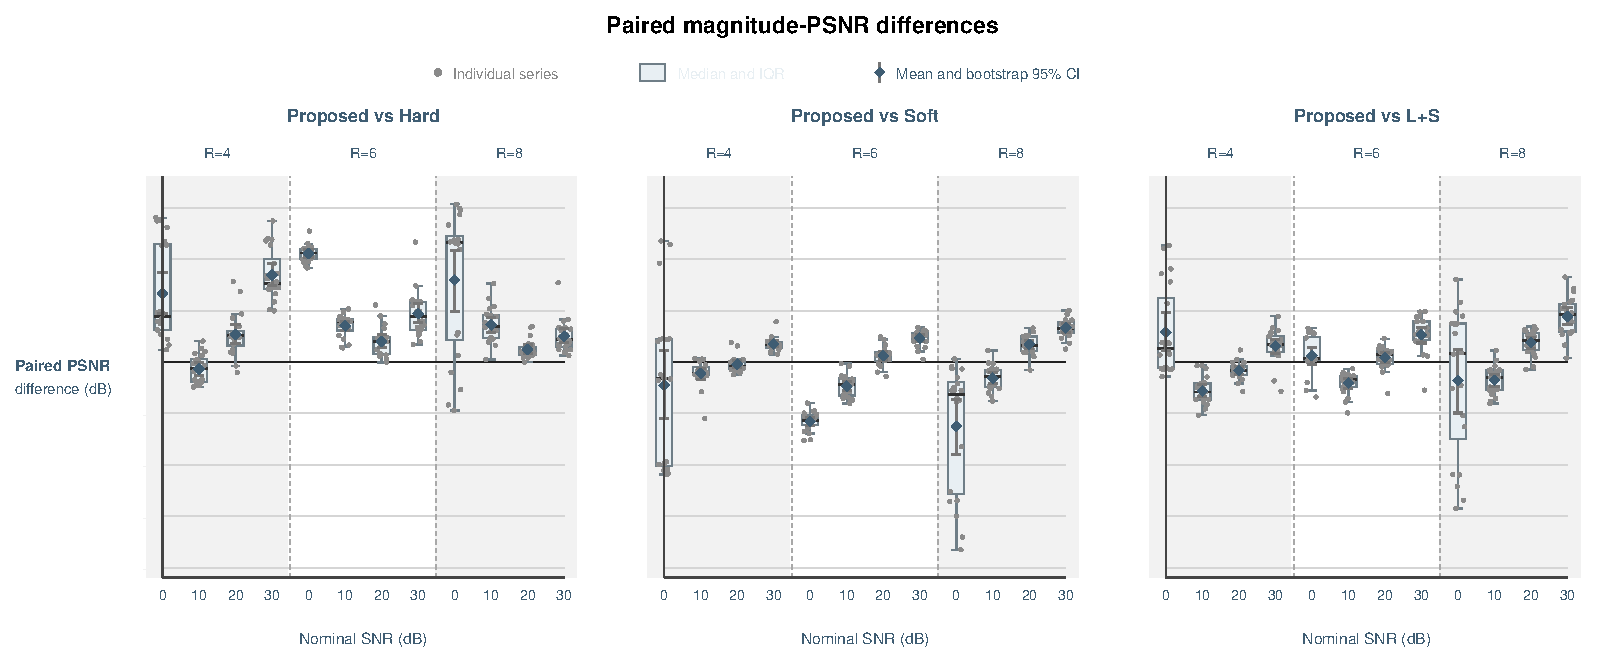
\includegraphics[width=\textwidth]{fig4_paired_psnr_distributions.pdf}
  \caption{20 个正式序列的配对幅值 PSNR 差。正值表示 Proposed 更优。图中同时显示个体序列、 中位数、四分位区间、均值和 95\% 配对 bootstrap 区间。}
  \label{fig:paired_psnr_distributions_zh}
\end{figure*}

图~\ref{fig:secondary_metrics_zh} 中的补充指标支持相同的条件依赖结论。相对于 Hard，NMSE 与 SSIM 多数有利于 Proposed 或接近中性；相对于 Soft 和 L+S，两项指标的方向总体上与 PSNR 的交叉变化一致，而最强噪声下区间最宽。这些指标用于验证结论一致性，而不是第二组选参目标。

\begin{figure*}[t]
  \centering
  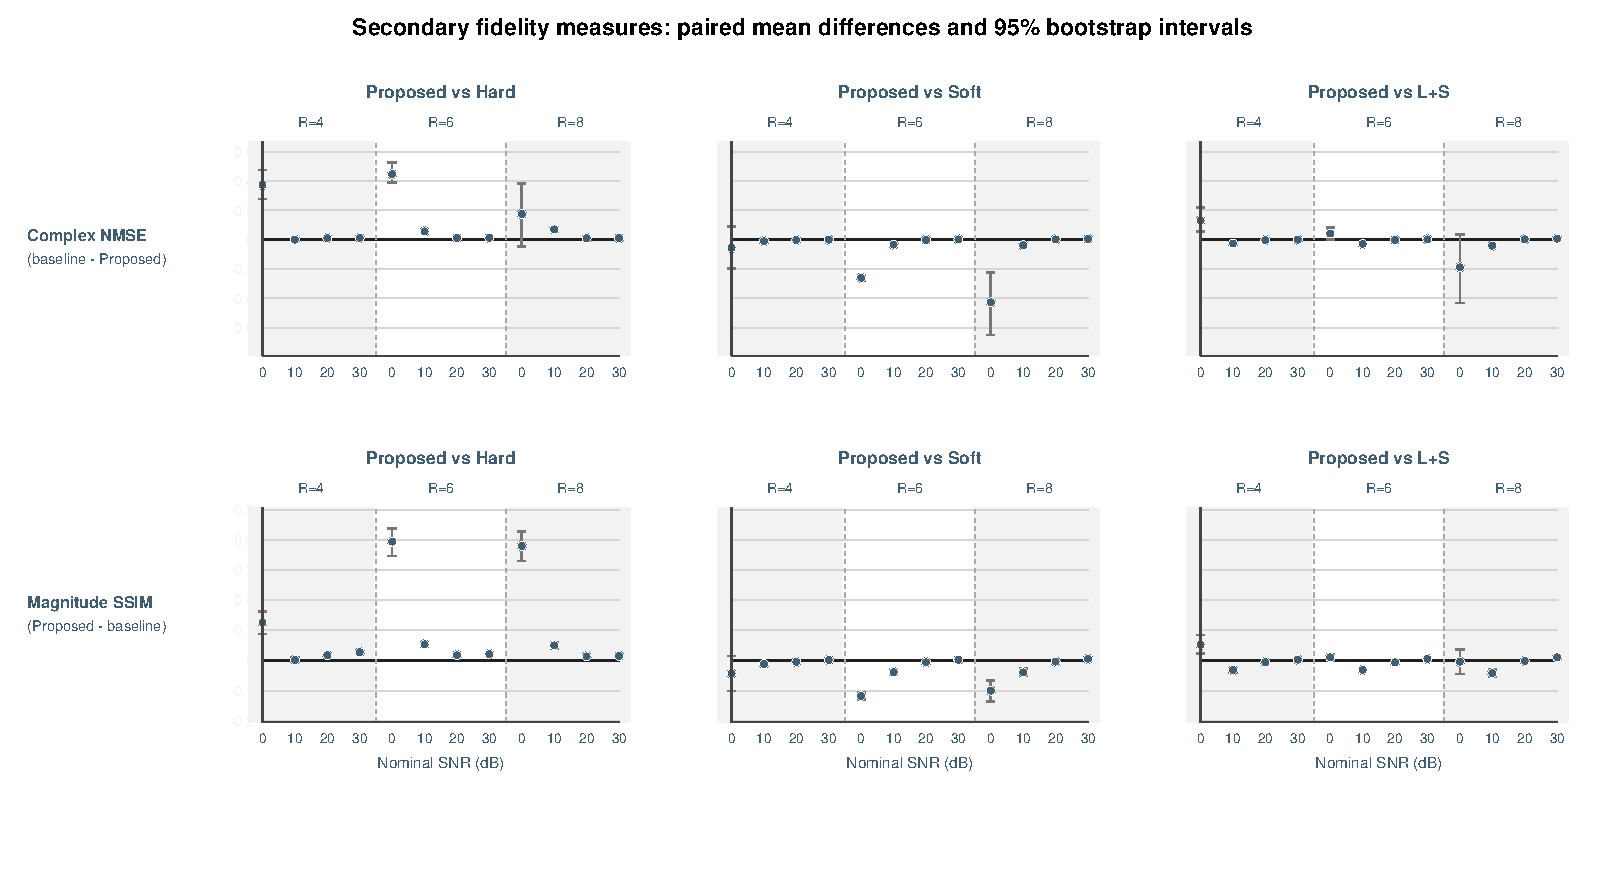
\includegraphics[width=\textwidth]{fig5_secondary_metric_intervals.pdf}
  \caption{复数 NMSE 与幅值 SSIM 的配对均值差和 95\% 配对 bootstrap 区间。NMSE 定义为基线减 Proposed，SSIM 定义为 Proposed 减基线，因此两行中正值均表示 Proposed 更优。该低饱和度点区间图取代按指标单独设色的热图。}
  \label{fig:secondary_metrics_zh}
\end{figure*}

图~\ref{fig:qualitative_temporal_zh} 给出两个预先按“最接近条件中位差”选定的例子：$R=4$、0~dB 下的 Proposed--Soft 比较，以及 $R=8$、30~dB 下的 Proposed--L+S 比较。每组包含参考图像、当前帧采样掩膜、含噪零填充图像、四种重建结果和采用 jet 色图的绝对误差图。参考图像与掩膜下方的误差单元格留空。该图展示强噪声下 Soft 的稳定性与低噪声下 Proposed 较小的收缩偏差，但不以两个个例替代总体统计证据。

\begin{figure*}[p]
  \centering
  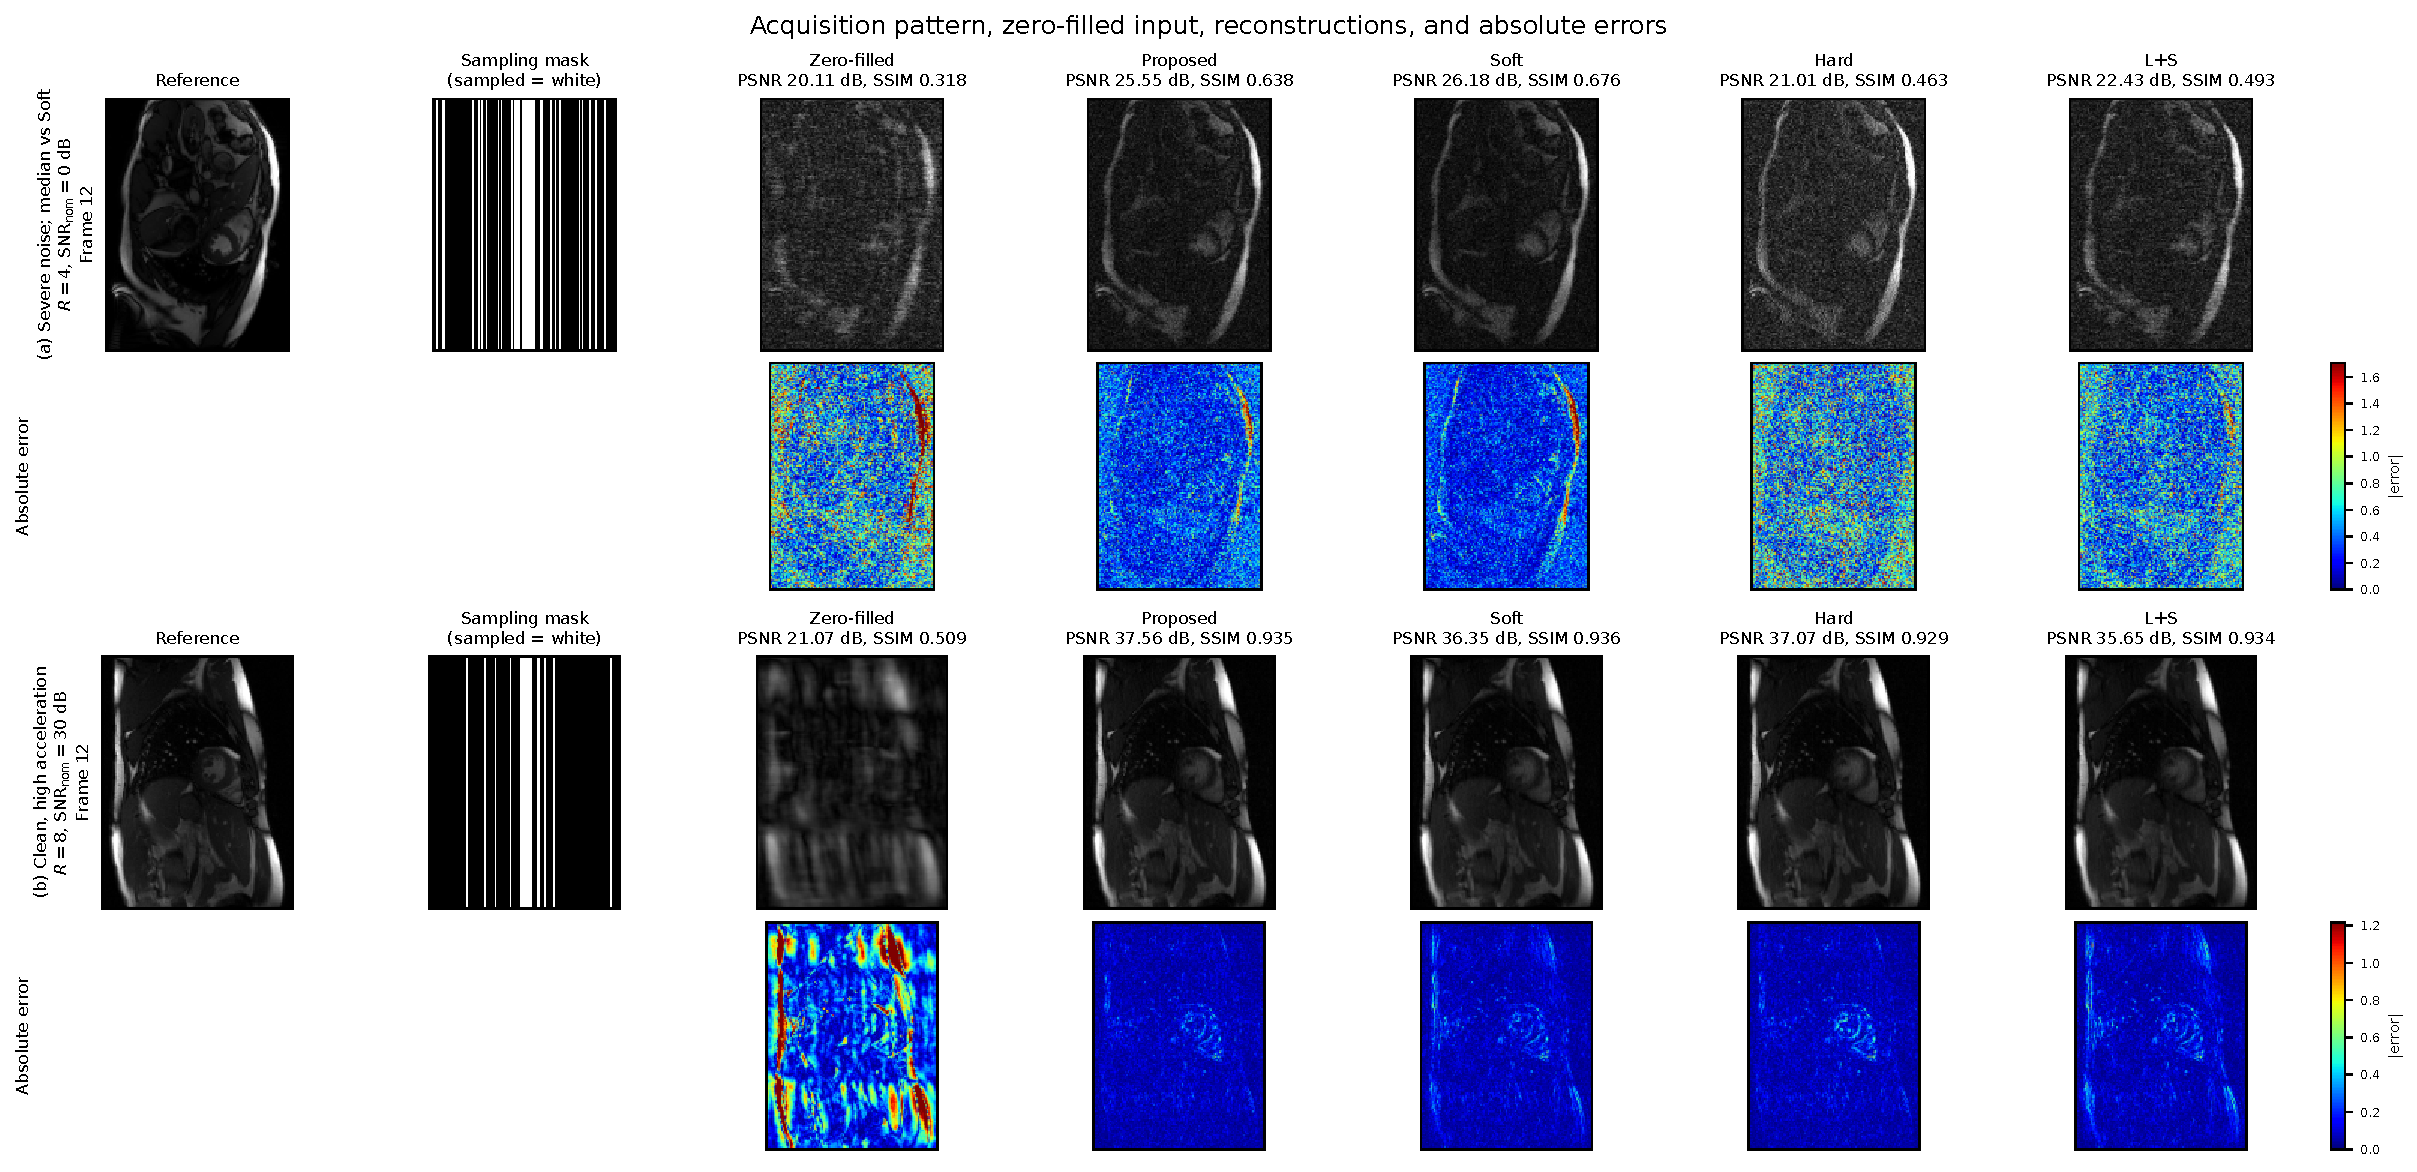
\includegraphics[width=\textwidth]{fig6_qualitative_temporal_comparison.pdf}
  \caption{参考图像、采样掩膜（白色表示已采相位编码位置）、含噪零填充输入、重建结果与幅值绝对误差图。(a) $R=4$、$\mathrm{SNR}_{\mathrm{nom}}=0$~dB；(b) $R=8$、$\mathrm{SNR}_{\mathrm{nom}}=30$~dB。显示中间心动时相，PSNR 与 SSIM 按完整电影序列计算。}
  \label{fig:qualitative_temporal_zh}
\end{figure*}

\subsection{实验流程诊断}
\label{sec:protocol_diagnostics_zh}

\subsubsection{仅使用 pilot 数据的参数边界审计}
\label{sec:boundary_audit_zh}

仅当某个 pilot 序列的验证最优候选位于参数下边界或上边界，且其相对于相邻内部候选的改善超过数值容差时，才沿对应坐标向外扩展参数范围，同时固定其余坐标。新增候选继续使用相同的掩膜、噪声、验证划分和停止规则。6 轮审计共评估 97 个向外扩展设置，即 388 次 pilot 重建，未出现失败；第 6 轮结束后没有新的触发项。随后，候选集在正式实验前冻结。20 个正式序列不参与任何边界驱动的范围调整，否则会使选参空间适应评估数据。在冻结的 300 次迭代流程下，无需继续增加边界实验；如果改变停止准则或选参流程，则必须重新进行边界审计。

\subsubsection{收敛性与迭代上限敏感性}
\label{sec:convergence_sensitivity_zh}

在 300 次以内达到相对迭代变化阈值的正式重拟合数量分别为：Proposed 74/240、Soft 175/240、Hard 238/240、L+S 40/240；其余运行在共同上限处停止。因此，主要实验比较的是预先规定的早停流程，而非各方法完全收敛后的全局最优解。

在固定已选参数的前提下，将代表性运行继续至最多 600 次。对于 $R\in\{4,8\}$、$\mathrm{SNR}_{\mathrm{nom}}\in\{0,30\}$~dB 四个角点条件中的 Proposed 与 L+S，8 个运行均在 600 次前达到阈值，最大绝对 PSNR 变化为 0.104~dB，且四个 Proposed--L+S 排序均未改变。对于针对性的 $R=4$、10~dB Proposed--Hard 个例，差值由 $-0.139$ 变为 $-0.855$~dB，原因是 Proposed 下降 0.716~dB，而 Hard 在第 140 次收敛后保持不变。因此，该正式实验中的单一反转不能解释为迭代上限偏向 Hard。由于迭代上限与选参共同定义完整方法，主要实验保留 300 次上限；若改用 600 次作为正式流程，则需要重新进行 pilot 选参和边界审计。

\begin{figure*}[t]
  \centering
  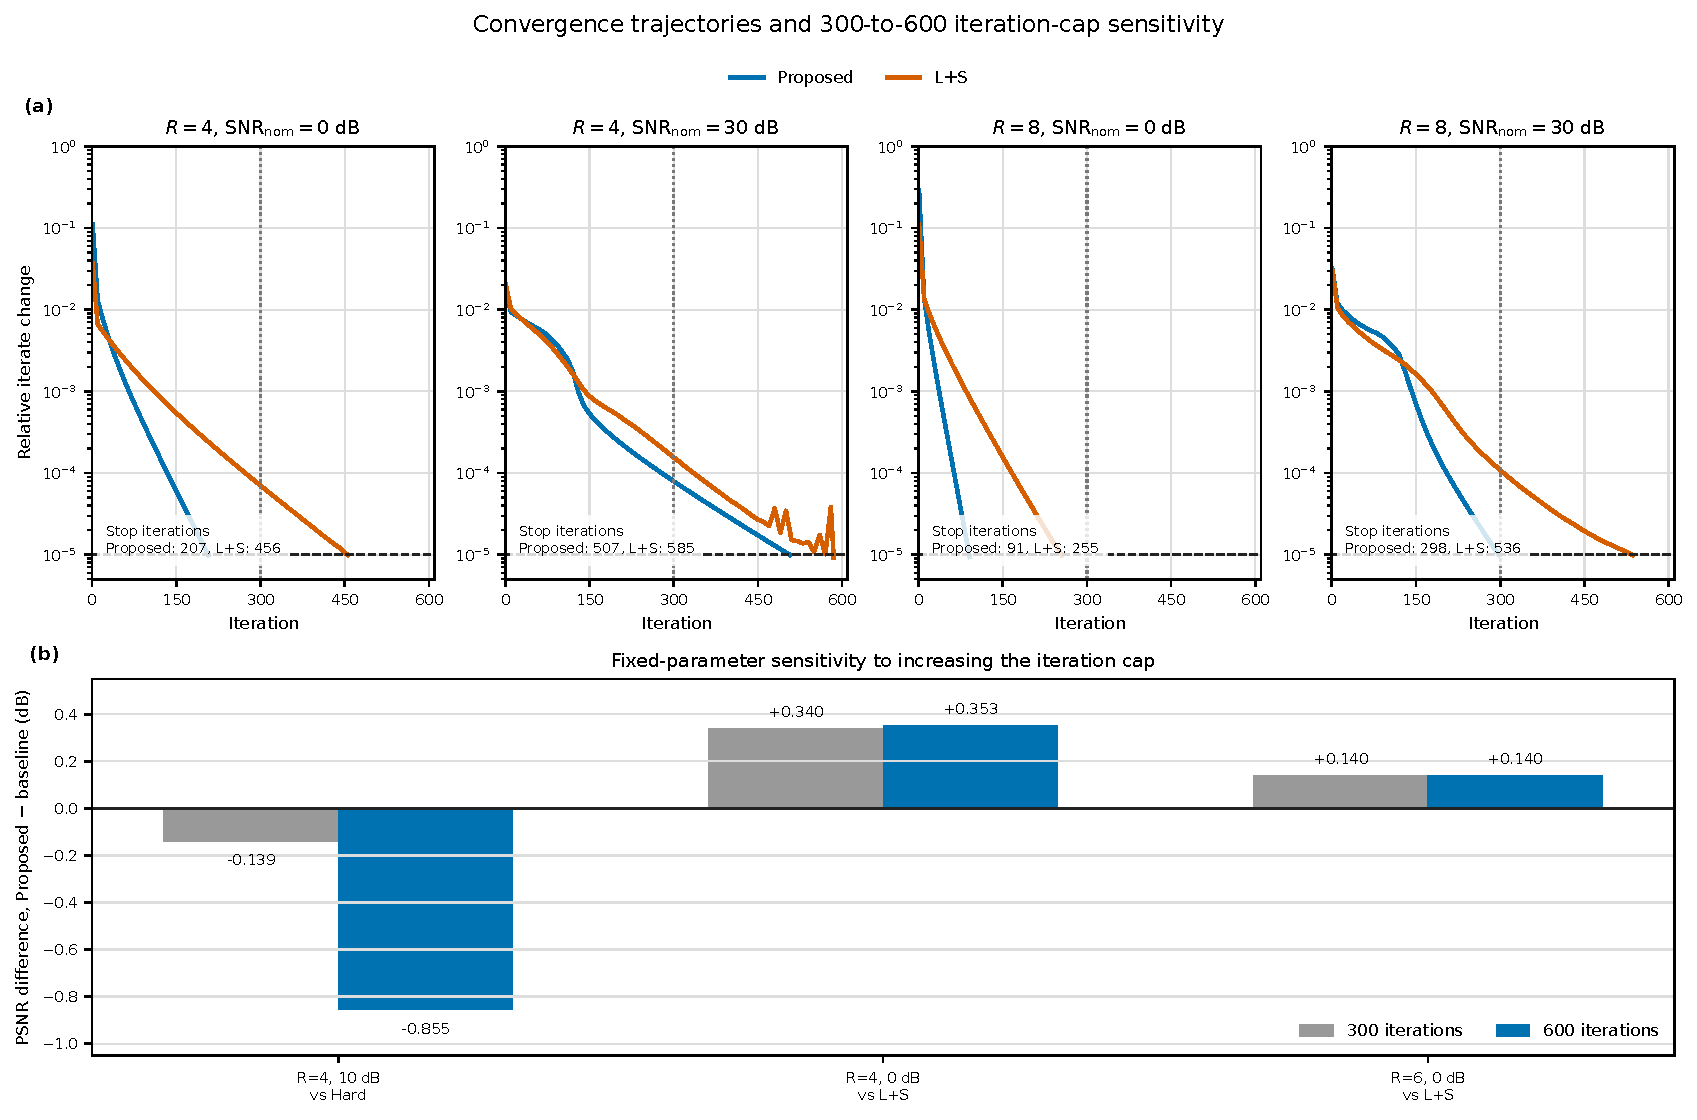
\includegraphics[width=\textwidth]{fig3_convergence_sensitivity.pdf}
  \caption{收敛性与迭代上限敏感性。图中给出代表性 Proposed/L+S 角点条件的相对迭代变化，以及针对性比较中 300 次和 600 次时的 Proposed 减基线 PSNR 差。继续迭代时参数保持不变。}
  \label{fig:convergence_sensitivity_zh}
\end{figure*}

\subsection{讨论与局限性}
\label{sec:evaluation_discussion_zh}

总体而言，Proposed 通常优于 Hard，而相对于 Soft 与 L+S 呈现明确的条件依赖权衡。0--10~dB 时，更强或更传统的收缩往往更稳定；20~dB 时 Proposed 开始具有竞争力；30~dB 时 Proposed 在三个加速倍数的 PSNR 上均占优。该现象与低噪声下主要时间奇异分量的收缩偏差减小相一致，但本实验不能对这一机制给出因果证明。0~dB 的非单调结果也具有合理性：按噪声构造，已采信号与新增噪声的 RMS 相等，此时解剖结构、采样掩膜和含噪验证选择之间的相互作用会产生更宽且更偏斜的配对差值。

本研究仅包含 20 个 OCMR 序列，且无法确认患者层面的独立性。欠采样与高斯噪声均为回顾性模拟，ESPIRiT 图和参考图像又在降质前由全采样数据获得。线圈合成还使结论仅适用于本文的单图像流程，而不能直接推广至灵敏度编码的多线圈重建。候选集由 4 个 pilot 序列构建，收敛性分析也只覆盖代表性个例而非全部正式数据。最后，NMSE、PSNR 与 SSIM 的改善尚未通过盲法阅片或临床任务验证。在这些限制下，实验支持 Proposed 在大多数条件下相对于 Hard 的稳定优势，以及其相对于 Soft 和 L+S 的噪声依赖优势，而不支持无条件的普遍优越性。
